% !TEX root = mythesis.tex

%==============================================================================
\chapter{Dark Photon $A'$}
\label{sec:darkp}
%==============================================================================
This section describes the theory and motivation for a new U(1) gauge boson that couples to the SM via kinetic mixing with the photon. The first indication of the existence of such a light boson was arrived at as an attempt to explain the astrophysical observations especially from PAMELA and WMAP/PLANCK. The explanation for the observed results was dark matter annihilation into $e^+e^-$. The PAMELA results required a large cross-section into leptons and a low cross-section into hadrons for the theorized particle. Taking this observation and building a model~\cite{Arkani_Hamed_2009} for this hypothesized particle already helped negate a few SM candidates such as Z, W and Higgs bosons (all (three) have low cross-section into leptons) and thermal WIMP (low cross-section at small lorentz boosts)~\cite{Arkani_Hamed_2009}, which is a competing dark matter prospect. Occurrence of a light vector boson that annihilates to leptons might explain these observations. Such a boson $A'$ was added to the SM in the simplest way by introducing a new spontaneously broken U(1) gauge field which couples via kinetic mixing with the ordinary photon, first discussed in \cite{HOLDOM1986196,GALISON1984279}. The Lagrangian is modified in the following way:
\begin{equation}\label{eq:Lagrangian}
  {\cal L} =  L_{SM} - \frac{1}{4} F'_{\mu\nu}F^{\mu\nu} + \frac{\epsilon}{2} F'_{\mu\nu}F^{\mu\nu} + \frac{m^2_{A'}}{2} A'_{\mu}A^{\mu} + i \overline{\chi} \gamma^{\mu} \partial_{\mu} \chi - m_{\chi} \overline{\chi} \chi - e_D \overline{\chi} \gamma^{\mu} A'_{\mu} \chi
\end{equation}
here $A'_{\mu}$ is the field associated with the dark photon, $\frac{\epsilon}{2} F'_{\mu\nu}F^{\mu\nu}$ is the kinetic mixing term between the dark photon and SM photon with $\epsilon$ describing the mixing strength. $\chi$ is treated as a placeholder for dark matter fermions which couple to $A'$ via the coupling constant $e_D$ also known as the dark portal coupling constant, $m_{A'}$ and $m_{\chi}$ are the masses of the $A'$ and the dark matter fermion respectively. The $A'$ can aquire its mass via the Higgs~\cite{PhysRevLett.13.508} or the Stueckelberg~\cite{Kors:2005uz} mechanism.

The mixing between the SM photon and $A'$ offers a possible channel for its production such as the high energy electron scattering off a nuclei $e^-Z\rightarrow e^- Z A'$. The production cross-section of $A'$ for this reaction was calculated using improved Weizsäker-Williams (IWW) approximation and the exact tree-level (ETL) calculations by Liu et al. \cite{Liu:2017htz} and Gninenko et al. \cite{Gninenko:2017yus}. This calculation is extremely important since it gives us a theoretical prediction for the number of $A's$ that could be produced for this channel and is also useful for the implementation of a MC simulation for the reaction.

\begin{figure}[t!]
\centering
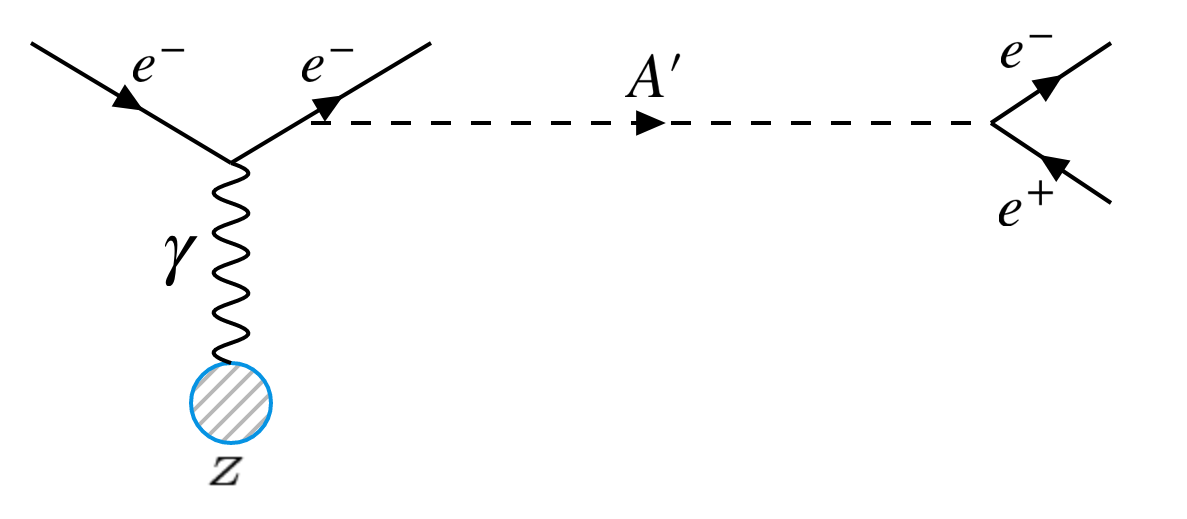
\includegraphics[width=14.5cm]{thesis_figures/VISIBLE.png}
\caption{Visible mode }
\label{fig:Visible_feynman}
\end{figure}

\begin{figure}[t!]
\centering
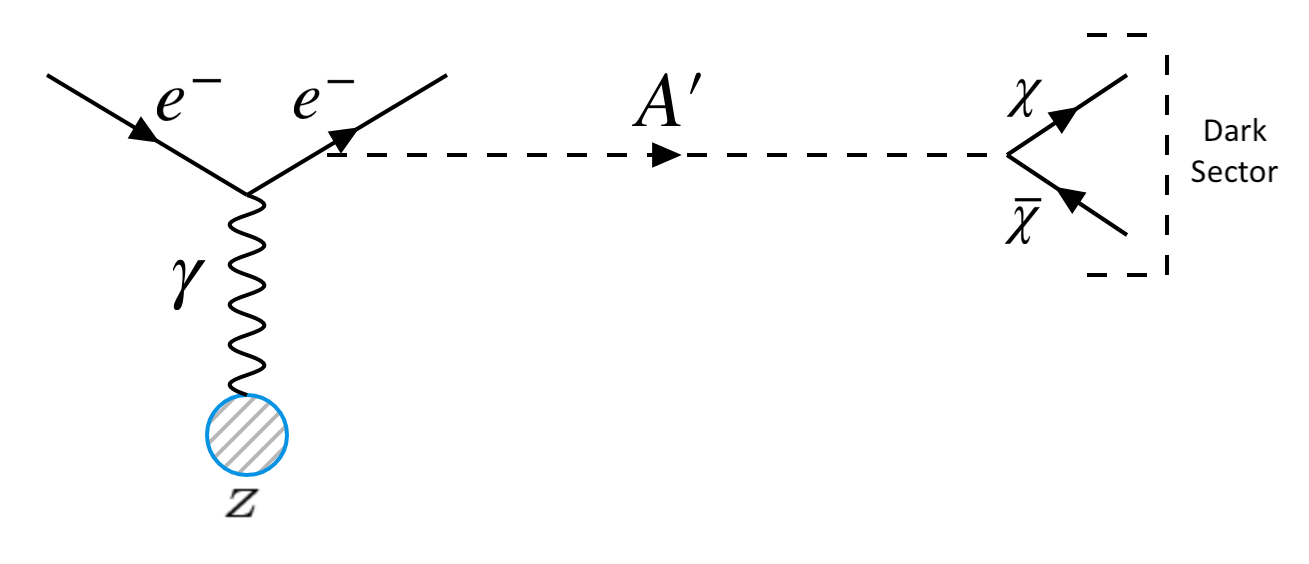
\includegraphics[width=15cm]{thesis_figures/INVISIBLE.png}
\caption{Invisible mode }
\label{fig:Invisible_feynman}
\end{figure}
Clearly from eq.(\ref{eq:Lagrangian}) there are two possibilities for the detection of $A'$. It can be either observed via its decay to SM particles which is called the \textit{visible mode} (fig.(\ref{fig:Visible_feynman})) or via its decay to light DM particles known as the \textit{invisible mode} (fig.(\ref{fig:Invisible_feynman})). In the visible mode we assume that $A'$ is one of the lightest states in the dark sector, then it is fair to believe that it would mainly decay to SM leptons. Such an interaction is described by the Lagrangian ${\cal L}_{int} = \epsilon e A'_{\mu} J^{\mu}_{em}$ where $J^{\mu}_{em}$ is the electromagnetic current and $e$ is the electromagnetic coupling. Such a decay would assume the $A'$ to have a sub-GeV mass and $\epsilon \ll 1 $. It also allows for an opportunity to set up an experiment for this particular mode since we will directly observe an excess of leptons in the final state. On the other hand for the invisible mode we assume that $A'$ is not the lightest state and there exists some other state $\chi$ with a lower mass, such that $A'\rightarrow \chi \overline{\chi}$ is a possibility. Such an event can also be probed with a so called missing energy experiment where the produced $A'$ or $\chi$ carries away some of the energy and is not detected.

The production and detection mechanisms discussed offer us the basic ingredients needed to set up an experiment for the detection of $A'$. One of the simpler layouts for such an experiment is an electron beam dump experiment. NA64 falls in this category, the setup of which is discussed in the next chapter.
\begin{figure}[t!]
\centering
  \begin{minipage}[t]{.45\textwidth}
    \centering
    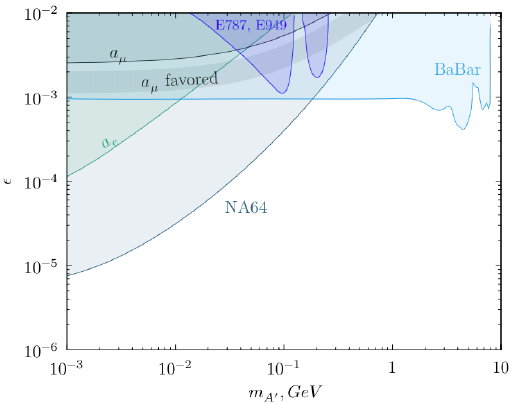
\includegraphics[width=\textwidth]{thesis_figures/exclusion_invisible.png}
    \caption{Current limits for invisible mode for 90\% C.L. exclusion region in the ($m_{A'},\epsilon$) plane ~\cite{2019EPJWC.21206005K}.}
    \label{fig:exclusion_invisible}
  \end{minipage}
  \hfill
  \begin{minipage}[t]{.45\textwidth}
    \centering
    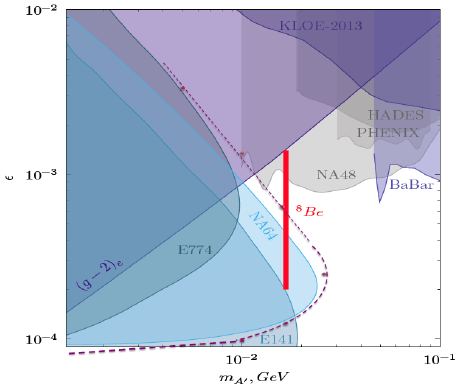
\includegraphics[width=\linewidth]{thesis_figures/exclusion_visible_latest.png}
    \caption{Current limits for invisible mode for 90\% C.L. exclusion region in the ($m_{A'},\epsilon$) plane. The blue plane is with 2017 data and the dotted line is with 2017+2018 data for NA64. The red line is the region that might explain the X17 boson~\cite{2019EPJWC.21206005K}.}
    \label{fig:exclusion_visible}
  \end{minipage}
\end{figure}


%%% Local Variables:
%%% mode: latex
%%% TeX-master: "mythesis"
%%% End:
